
%% bare_jrnl_compsoc.tex
%% V1.4a
%% 2014/09/17
%% by Michael Shell
%% See:
%% http://www.michaelshell.org/
%% for current contact information.
%%
%% This is a skeleton file demonstrating the use of IEEEtran.cls
%% (requires IEEEtran.cls version 1.8a or later) with an IEEE
%% Computer Society journal paper.
%%
%% Support sites:
%% http://www.michaelshell.org/tex/ieeetran/
%% http://www.ctan.org/tex-archive/macros/latex/contrib/IEEEtran/
%% and
%% http://www.ieee.org/

%%*************************************************************************
%% Legal Notice:
%% This code is offered as-is without any warranty either expressed or
%% implied; without even the implied warranty of MERCHANTABILITY or
%% FITNESS FOR A PARTICULAR PURPOSE! 
%% User assumes all risk.
%% In no event shall IEEE or any contributor to this code be liable for
%% any damages or losses, including, but not limited to, incidental,
%% consequential, or any other damages, resulting from the use or misuse
%% of any information contained here.
%%
%% All comments are the opinions of their respective authors and are not
%% necessarily endorsed by the IEEE.
%%
%% This work is distributed under the LaTeX Project Public License (LPPL)
%% ( http://www.latex-project.org/ ) version 1.3, and may be freely used,
%% distributed and modified. A copy of the LPPL, version 1.3, is included
%% in the base LaTeX documentation of all distributions of LaTeX released
%% 2003/12/01 or later.
%% Retain all contribution notices and credits.
%% ** Modified files should be clearly indicated as such, including  **
%% ** renaming them and changing author support contact information. **
%%
%% File list of work: IEEEtran.cls, IEEEtran_HOWTO.pdf, bare_adv.tex,
%%                    bare_conf.tex, bare_jrnl.tex, bare_conf_compsoc.tex,
%%                    bare_jrnl_compsoc.tex, bare_jrnl_transmag.tex
%%*************************************************************************


% *** Authors should verify (and, if needed, correct) their LaTeX system  ***
% *** with the testflow diagnostic prior to trusting their LaTeX platform ***
% *** with production work. IEEE's font choices and paper sizes can       ***
% *** trigger bugs that do not appear when using other class files.       ***                          ***
% The testflow support page is at:
% http://www.michaelshell.org/tex/testflow/


\documentclass[10pt,conference,onecolumn,compsoc]{IEEEtran}


\usepackage{hyperref}
\usepackage{enumitem}
\setlist[itemize]{leftmargin=3 cm}
\setlist[enumerate]{leftmargin=3cm}



% *** CITATION PACKAGES ***
%
\ifCLASSOPTIONcompsoc
  % IEEE Computer Society needs nocompress option
  % requires cite.sty v4.0 or later (November 2003)
  \usepackage[nocompress]{cite}
\else
  % normal IEEE
  \usepackage{cite}
\fi
% cite.sty was written by Donald Arseneau
% V1.6 and later of IEEEtran pre-defines the format of the cite.sty package
% \cite{} output to follow that of IEEE. Loading the cite package will
% result in citation numbers being automatically sorted and properly
% "compressed/ranged". e.g., [1], [9], [2], [7], [5], [6] without using
% cite.sty will become [1], [2], [5]--[7], [9] using cite.sty. cite.sty's
% \cite will automatically add leading space, if needed. Use cite.sty's
% noadjust option (cite.sty V3.8 and later) if you want to turn this off
% such as if a citation ever needs to be enclosed in parenthesis.
% cite.sty is already installed on most LaTeX systems. Be sure and use
% version 5.0 (2009-03-20) and later if using hyperref.sty.
% The latest version can be obtained at:
% http://www.ctan.org/tex-archive/macros/latex/contrib/cite/
% The documentation is contained in the cite.sty file itself.



% *** GRAPHICS RELATED PACKAGES ***
%
\ifCLASSINFOpdf
   \usepackage[pdftex]{graphicx}
 
\else
 
\fi
% graphicx was written by David Carlisle and Sebastian Rahtz. It is
% required if you want graphics, photos, etc. graphicx.sty is already
% installed on most LaTeX systems. The latest version and documentation
% can be obtained at: 
% http://www.ctan.org/tex-archive/macros/latex/required/graphics/
% Another good source of documentation is "Using Imported Graphics in
% LaTeX2e" by Keith Reckdahl which can be found at:
% http://www.ctan.org/tex-archive/info/epslatex/
%
% latex, and pdflatex in dvi mode, support graphics in encapsulated
% postscript (.eps) format. pdflatex in pdf mode supports graphics
% in .pdf, .jpeg, .png and .mps (metapost) formats. Users should ensure
% that all non-photo figures use a vector format (.eps, .pdf, .mps) and
% not a bitmapped formats (.jpeg, .png). IEEE frowns on bitmapped formats
% which can result in "jaggedy"/blurry rendering of lines and letters as
% well as large increases in file sizes.
%
% You can find documentation about the pdfTeX application at:
% http://www.tug.org/applications/pdftex









% *** PDF, URL AND HYPERLINK PACKAGES ***
%
\usepackage{url}
% url.sty was written by Donald Arseneau. It provides better support for
% handling and breaking URLs. url.sty is already installed on most LaTeX
% systems. The latest version and documentation can be obtained at:
% http://www.ctan.org/tex-archive/macros/latex/contrib/url/
% Basically, \url{my_url_here}.




\begin{document}

\title{Temtris}
%
%

% received ..."  text while in non-compsoc journals this is reversed. Sigh.

\author{Curt Lynch and Hunter Johnson}

\IEEEtitleabstractindextext{%
\begin{abstract}
Temtris is a Tetris-like we are developing as part of our CSCI352 class.
\end{abstract}
}

% make the title area
\maketitle

\IEEEdisplaynontitleabstractindextext

\IEEEpeerreviewmaketitle

\section{Introduction}
Temtris is a WPF clone of Tetris with our own spin added in. Tetris, is a game where 4 block section shapes fall from top down and you try to fit rows of these blocks together at an ever increasing pace until the screen inevitably fills causing game over. A score is computed based on how efficiently you clear the board as the game progresses, with more points being awarded for streaks of row clears and tetris row clears (4 simultaneous row clears). Our target audience is anyone looking to pass time with a casual game of Tetris. We are making Temtris as a duo as part of our CSCI 352 class. That being the case, we still want Temtris to be a fun and interesting game for anyone looking to play.

\subsection{Background}
A Tetrimino is one of the 7 classic Tetris shapes; these include the O, I, T, L, J, S, and Z shapes. Each Tetrimino is made up of four squares called minos. The matrix is the space where the Tetris game is played. A 'line clear' happens when a horizontal row is completely filled, causing it to be removed from the matrix. Lock-down is when a Tetrimino is locked into its current position and is no longer controllable.

While attempting to brainstorm ideas for our CSCI 352 class, the idea of a Tetris clone come up (with the awful misspelling Temtris). Eventually we settled on the idea and the name stuck.

\subsection{Impacts}
Tetris is a classic game that has had a major impact on the gaming community since its debut. Continuing to iterate upon Tetris and bring it back into the community repeatedly will only deepen its legacy. Temtris is a great way to  do this while improving our skills and preparing us for working in teams and on larger projects in the future.

\subsection{Challenges}
This is the first moderately sized project either of us has attempted. This is also our first real foray into WPF and c\# so there are some growing pains there as well. As for the project itself, I suspect getting the movement and rotations to feel like a proper Tetris game will take much more fine tuning than we have needed to use in the past. Rotating the pieces will likely also pose some sort of challenge.

\section{Scope}
Our initial goal is to implement the following typical parts of a Tetris-like: 
\begin{itemize}
\item Implement a main menu.
\item Have controllable tetriminos (2x1 shapes initially) that fall into place in the matrix. 
\item Have rows that disappear when they fill up, i.e., the line clears.
\item Keep score or track how well the player does in some way.
\item Display the next piece to spawn.
\end{itemize}

For stretch goals, we would like to add the following:
\begin{itemize}
\item Implement all 7 tetrimino variants.
\item Implement a multiplayer mode. Having at least two clients with a competitive game mode over LAN or just sharing a keyboard.
\item Different power-ups may be earned by removing a certain amount of one color from the board. Perhaps board clear (of that color) or maybe have the next five pieces all be 'L' shapes.
\item Play background music and have sound effects for line clears, player actions, etc.
\item Have random shapes form and fall into the matrix ( as opposed to the standard Tetris shapes.
\end{itemize}

\subsection{Requirements}
These requirements are things we feel make Tetris what it is. Without them the Temtris would ultimately not be a Tetris clone.

\subsubsection{Functional}
\begin{itemize}
\item Users can control Tetriminos (rotate, move left or right).
\item Tetriminos are created and fall from the top of the matrix.
\item Row clears should happen as the rows are filled.
\item Main menu allows the user to start the game.
\end{itemize}

\subsubsection{Non-Functional}
\begin{itemize}
\item Main menu should display controls needed to play the game.
\item User interface should be attractive and inviting.
\end{itemize}

\subsection{Use Cases}
\begin{table}[h!]
\centering
\begin{tabular}{|c|c|c|c|c|}
\hline
Use Case ID & Use Case Name & Primary Actor & Complexity & Priority \\
\hline \hline
1 & Start game & Player & Easy & 1\\
\hline
2 & Move tetriminos left or right & Player & Easy & 1\\
\hline
3 & Lower tetrimonios into position & Player & Med & 2\\
\hline
4 & Rotate tetriminos & Player & Hard & 3\\
\hline
\end{tabular}
\caption{use case table}
\label{tab:useCaseIndex}
\end{table}

\begin{itemize}
\item[Use Case Number:] 1
\item[Use Case Name:] Start game
\item[Description:] A player wishes to pass some time by playing Temptris. They start the game and click on the "Start Game" button from the main menu.
\end{itemize}
\begin{enumerate}
\item The Player launches the application.
\item The Player left-clicks on "Start Game" button.
\item The game screen appears and the game begins.
\item[Termination Outcome:] A game of Temtris is now running.
\end{enumerate}
Alternative: A previous game of Temtris has just ended.
\begin{enumerate}
\item Player left-clicks on "Play Again" button.
\item The game screen appears and the game begins..
\item[Termination Outcome:] A game of Temtris is now running.
\end{enumerate}
\medskip
 
\begin{itemize}
\item[Use Case Number:] 2
\item[Use Case Name:] Move tetriminos left or right
\item[Description:] A game of Temtris has been started and the player wishes to move the falling piece to the left or right. The player presses the left or right arrow on the keyboard and the active tetrimino moves accordingly.
\end{itemize}
\begin{enumerate}
\item The player presses the left arrow key on the keyboard.
\item The active tetrimino shifts one position to the left.
\item Player presses the right arrow key on the keyboard.
\item The active tetrimino shifts one block to the right.
\item[Termination Outcome:] The player has control over the left and right motion of the active tetrimino.
\end{enumerate}
\medskip

\begin{itemize}
\item[Use Case Number:] 3
\item[Use Case Name:] Lower tetriminos into position
\item[Description:] The player is comfortable with the current trajectory of the active tetrimino and wishes to lower it into place. The player presses the down arrow key on the keyboard and the active tetrimino moves down into place.
\end{itemize}
\begin{enumerate}
\item The player presses the down arrow key on the keyboard.
\item The active tetrimino begins to fall faster.
\item The active tetrimino stops falling when it reaches inactive tetriminos and is set into place.
\item[Termination Outcome:] The player can speed up the falling of the active tetrimino.
\end{enumerate}
\medskip
 
\begin{itemize}
\item[Use Case Number:] 4
\item[Use Case Name:] Rotate tetriminos
\item[Description:] The player wishes to rotate a tetrimino and presses the up arrow key on the keyboard. The active tetrimino rotates ninety degrees allowing the player to better control how it falls.
\end{itemize}
\begin{enumerate}
\item The player presses the up arrow key on the keyboard.
\item The active tetrimino rotates 90 degrees clockwise.
\item The player presses the up arrow key on the keyboard.
\item The active tetrimino rotates an additional 90 degrees clockwise.
\item[Termination Outcome:] The player has control over the rotation of the active tetrimino.
\end{enumerate}
\medskip

\subsection{Interface Mockups}

\begin{figure}[h!]
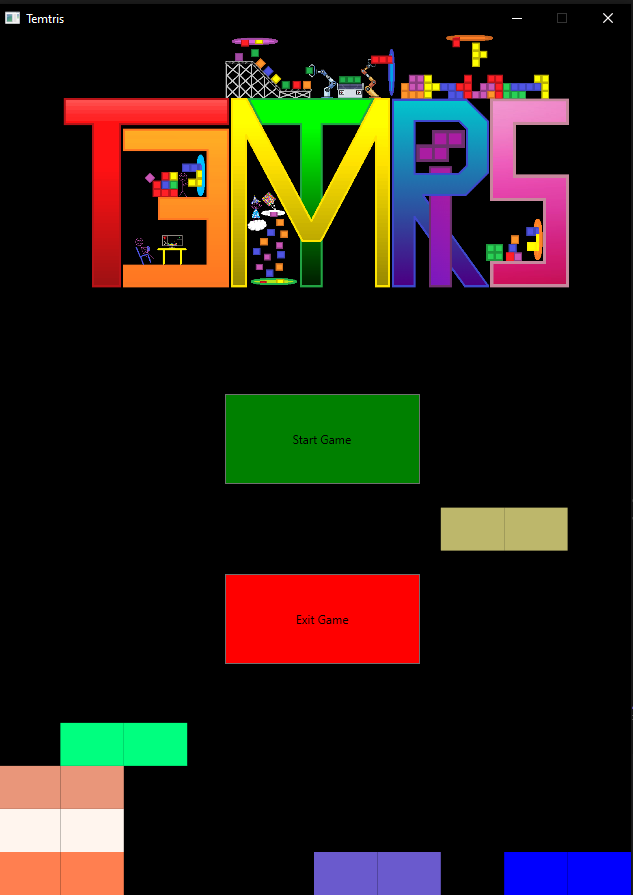
\includegraphics[scale=0.4]{MainMenu.png}
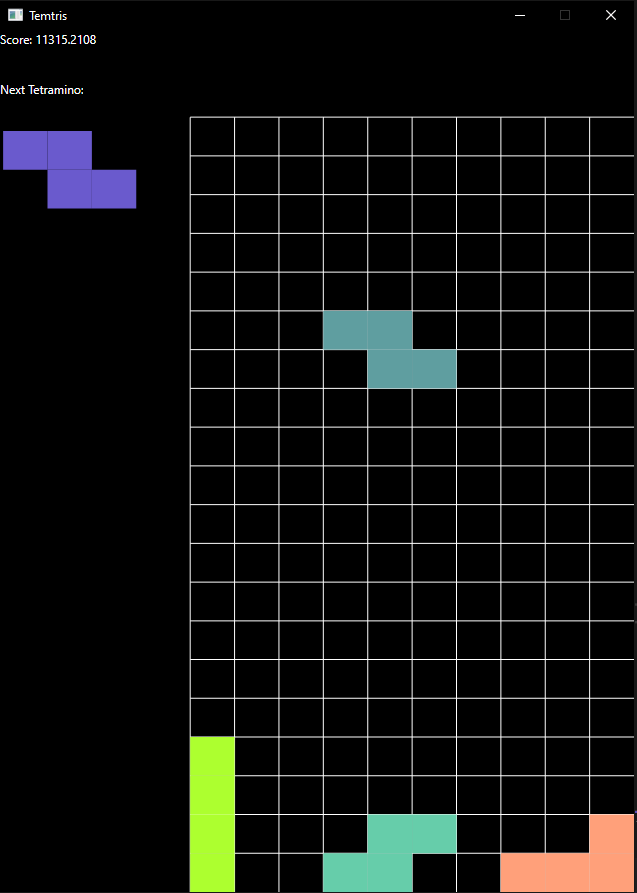
\includegraphics[scale=0.4]{GameRunning.png}
\caption{Temtris at the main menu(left) and during a game(right).}
\label{fig:uimockups}
\end{figure}

Todo: Tie interface mockups back into use cases and add game ending screen.
Figure \ref{fig:uimockups} shows various screenshots from Temtris as the user plays the game.

\section{Project Timeline}
\begin{figure}[h!]
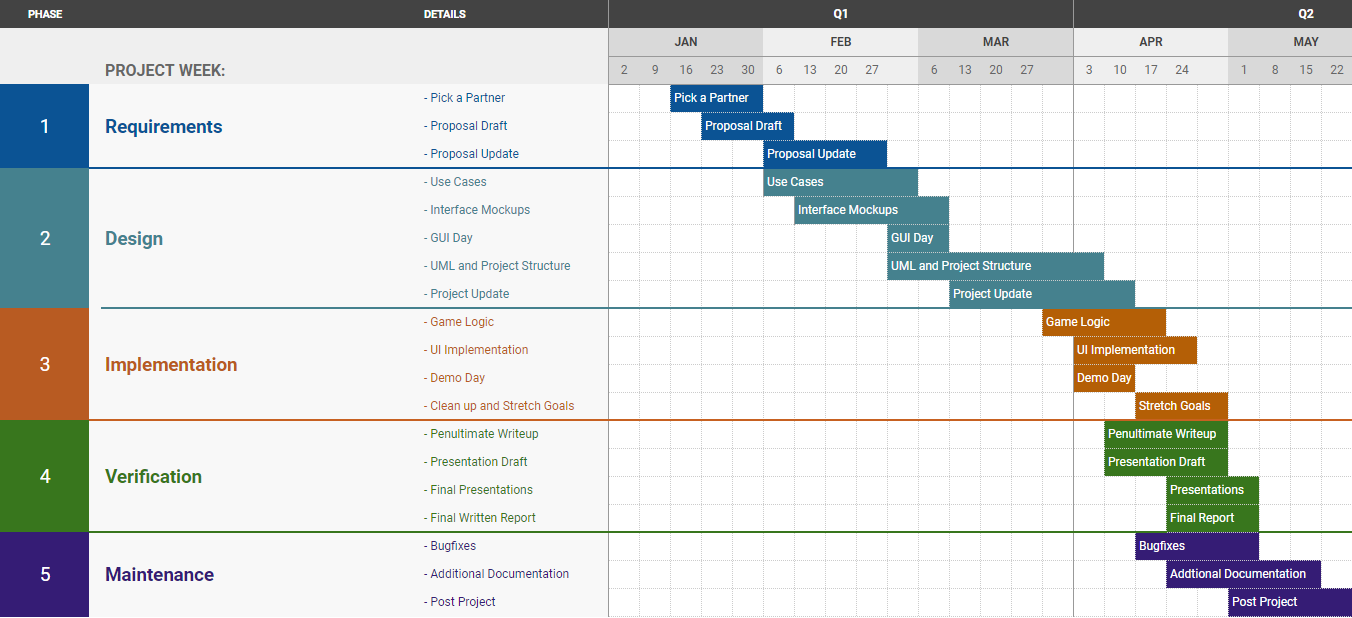
\includegraphics[scale=.45]{Timeline.png}
\caption{Project Timeline}
\end{figure}

As with most projects following the waterfall development cycle we wanted to solidify most of the design as early possible. This unfortunately left us with little time to actually implement the project and work out any rough edges in our design. If we had the chance to do this again we would've spent more time early learning WPF before attempting to outline a project using it. 

\section{Project Structure}

The UI exists within the auto generated MainWindow class, which calls upon an instantiation of the TemtrisGame class to handle all of the game logic and keyboard input.

\subsection{UML Outline}

\begin{figure}[h!]
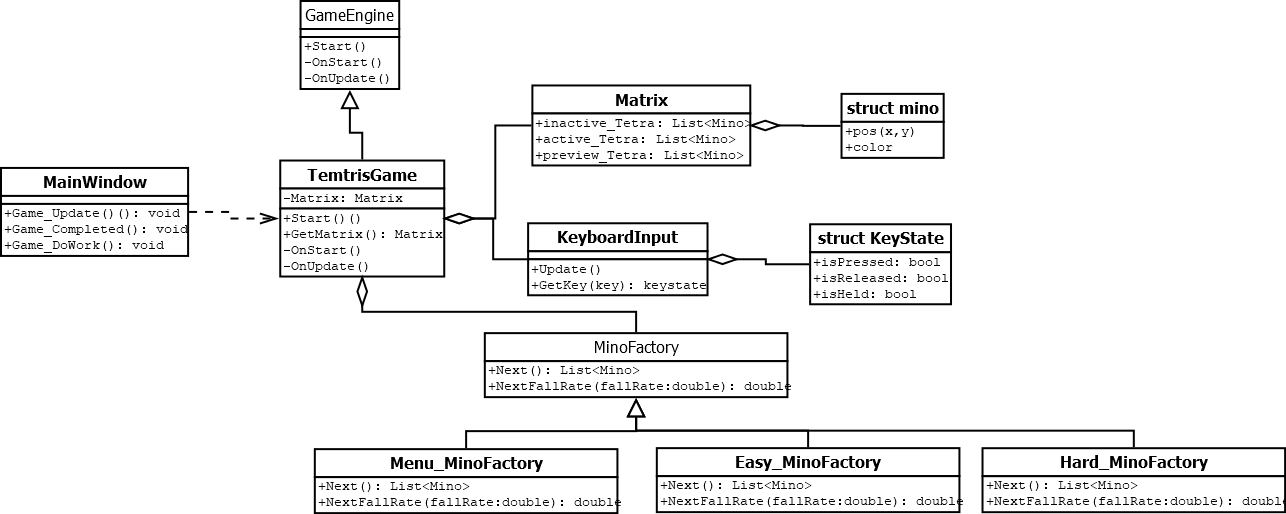
\includegraphics[scale=0.35]{TemtrisUML.png}
\caption{UML Diagram for Temtris}
\label{fig:uml}
\end{figure}

 Figure \ref{fig:uml} shows the breakdown of the class hierarchy for Temtris. \hfill\break
MainWindow: The auto generated class given when starting a WPF project in Visual Studio. This is the home of our UI. Utilizes TemtrisGame to get the layout and position of all Tetraminos.\hfill\break
GameEngine: This handles some of the more mundane non-Tetris aspects of the game engine.\hfill\break
TemtrisGame: The main Temtris class. Handles all of the game logic and keyboard input.\hfill\break
Matrix: A convenient data carrier. Stores all of the data for a given game data for a game of Temtris.\hfill\break
KeyboardInput: This keeps track of keyboard input and provides easy access to key state.\hfill\break
MinoFactory: Creates Tetraminos for the Tetris game, and provides updated fallRates. Each difficulty has it's own child class.\hfill\break


\subsection{Design Patterns Used}
TODO: clean up and explain a bit more.
There's a template pattern in there through GameEngine/TemtrisGame and an abstract factory pattern through MinoFactory.


\section{Results}
This section will start out a little vague, but it should grow as your project evolves.  With each deliverable you hand in, give me a final summary of where your project stands.  By the end, this should be a reflective section discussing how many of your original goals you managed to attain/how many desired use cases you implemented/how many extra features you added.

\subsection{Future Work}
Where are you going next with your project?
For early deliverables, what are your next steps?  (HINT: you will typically want to look back at your timeline and evaluate: did you meet your expected goals?  Are you ahead of schedule?  Did you decide to shift gears and implement a new feature?)
By the end, what do you plan on doing with this project?  Will you try to sell it?  Set it on fire?  Link to it on your resume and forget it exists?




\begin{thebibliography}{1}

\bibitem{IEEEhowto:kopka}
H.~Kopka and P.~W. Daly, \emph{A Guide to \LaTeX}, 3rd~ed.\hskip 1em plus
  0.5em minus 0.4em\relax Harlow, England: Addison-Wesley, 1999.

\end{thebibliography}



\begin{IEEEbiography}{Michael Shell}
Biography text here.
\end{IEEEbiography}

% if you will not have a photo at all:
\begin{IEEEbiographynophoto}{John Doe}
Biography text here.
\end{IEEEbiographynophoto}

% insert where needed to balance the two columns on the last page with
% biographies
%\newpage

\begin{IEEEbiographynophoto}{Jane Doe}
Biography text here.
\end{IEEEbiographynophoto}





% that's all folks
\end{document}


